\documentclass[12pt]{xtikzfig}
\newcommand{\col}{white}
\newcommand{\barthick}{0.016}
\newcommand{\barbasel}{0.0689}
\newcommand{\sqsize}{5.8}
\begin{document}%
  \begin{tikzpicture}%
    \node at (0,0) {%
      \begin{tikzpicture}%
        \node[anchor=south west,inner sep=0] (A) at (0,0) {%
          \fbox{\includegraphics[scale=0.075]{../src/A1/1A-0029.png}}};%
        \begin{scope}[x={(A.south east)},y={(A.north west)}]%
          \filldraw[fill=white,draw=white] (0.739,\barbasel) rectangle node[above] {%
            \footnotesize\color{\col}\SI{100}{\nano\metre}} +(0.195,\barthick);%
          \filldraw[fill=white,draw=black]%
           (0.01,0.89) rectangle +(0.1,0.1) node[pos=0.5] {\footnotesize (a)};%
          %\subfloat[\label{fig:a1_0030}TEM (BF) $\times$150k.]
        \end{scope}
      \end{tikzpicture}
    };
    %%%
    \node at (\sqsize,0) {  
      \begin{tikzpicture}    
        \node[anchor=south west,inner sep=0] (A) at (0,0) {%
          \fbox{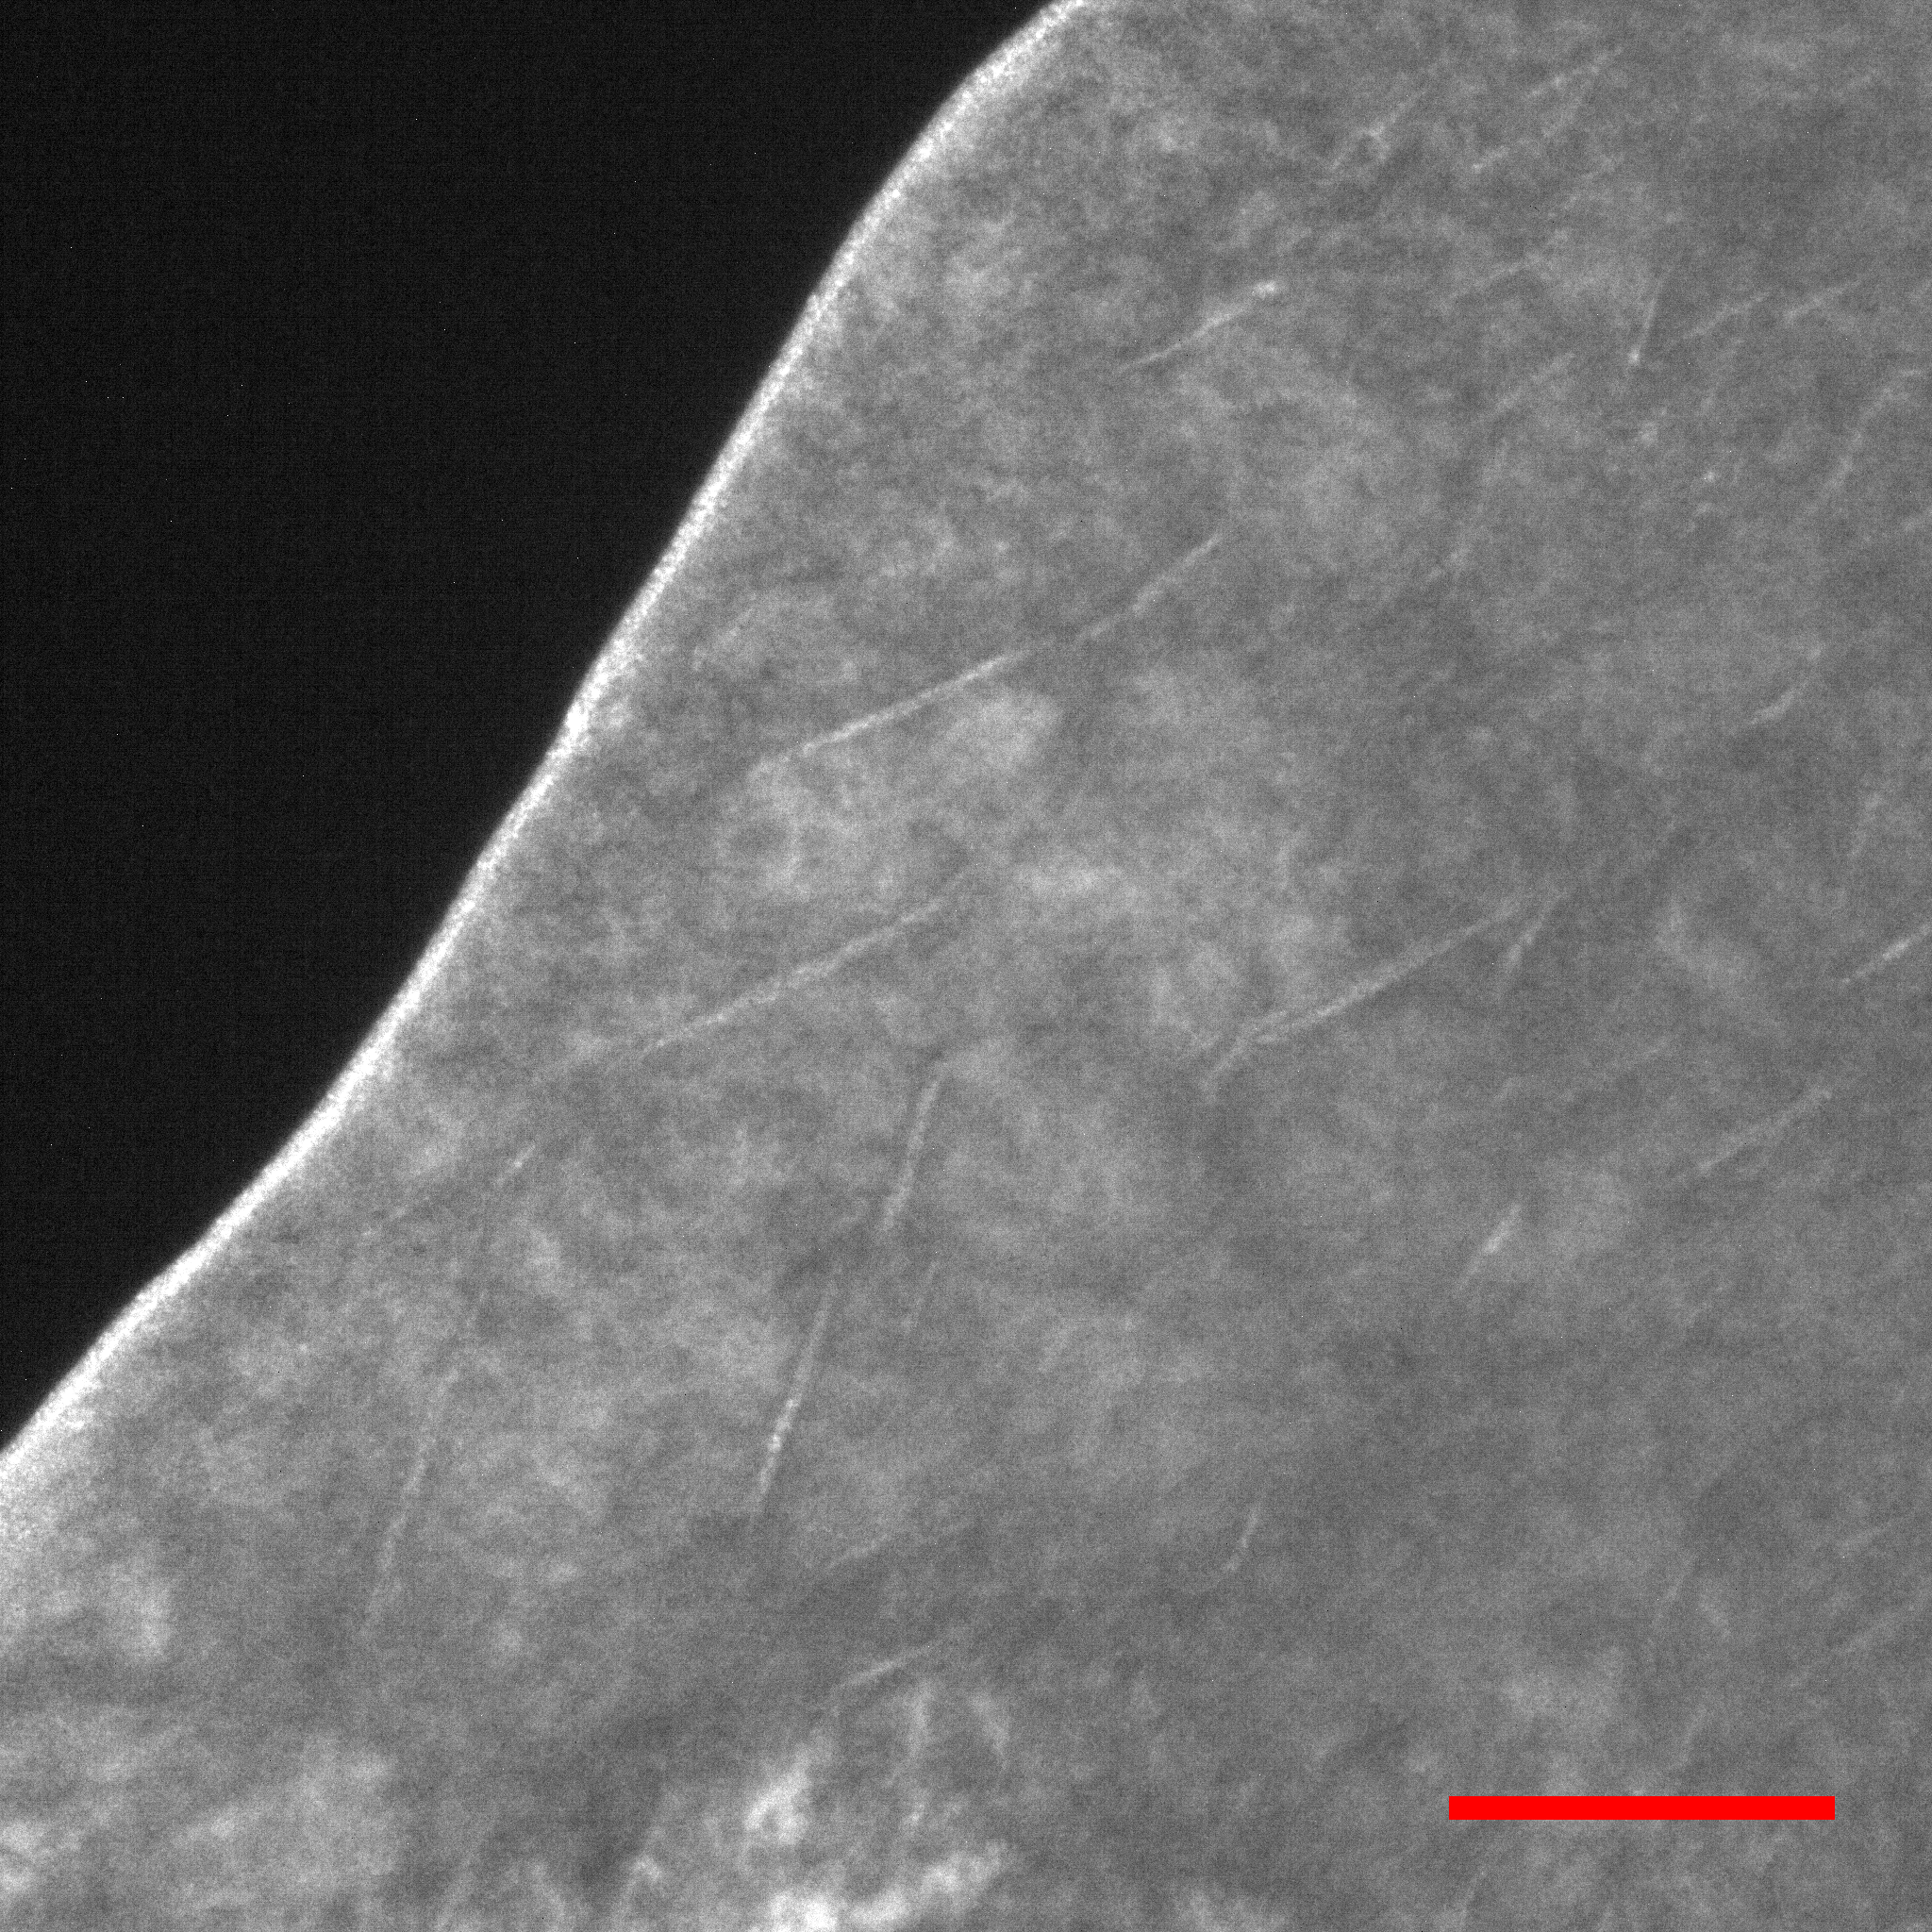
\includegraphics[scale=0.075]{../src/A1/1A-0030.png}}};
        \begin{scope}[x={(A.south east)},y={(A.north west)}]
          \filldraw[fill=white,draw=white] (0.739,\barbasel) rectangle node[above] {
            \footnotesize\color{\col}\SI{100}{\nano\metre}} +(0.195,\barthick);
          \filldraw[fill=white,draw=black] 
           (0.01,0.89) rectangle +(0.1,0.1) node[pos=0.5] {\footnotesize (b)}; 
          %\subfloat[\label{fig:a1_0030}TEM (DF) $\times$150k.]
        \end{scope}
      \end{tikzpicture}%
    };%
    %%%
    \node at (0,-\sqsize) {%
      \begin{tikzpicture}%    
      \node[anchor=south west,inner sep=0] (A) at (0,0) {%
        \fbox{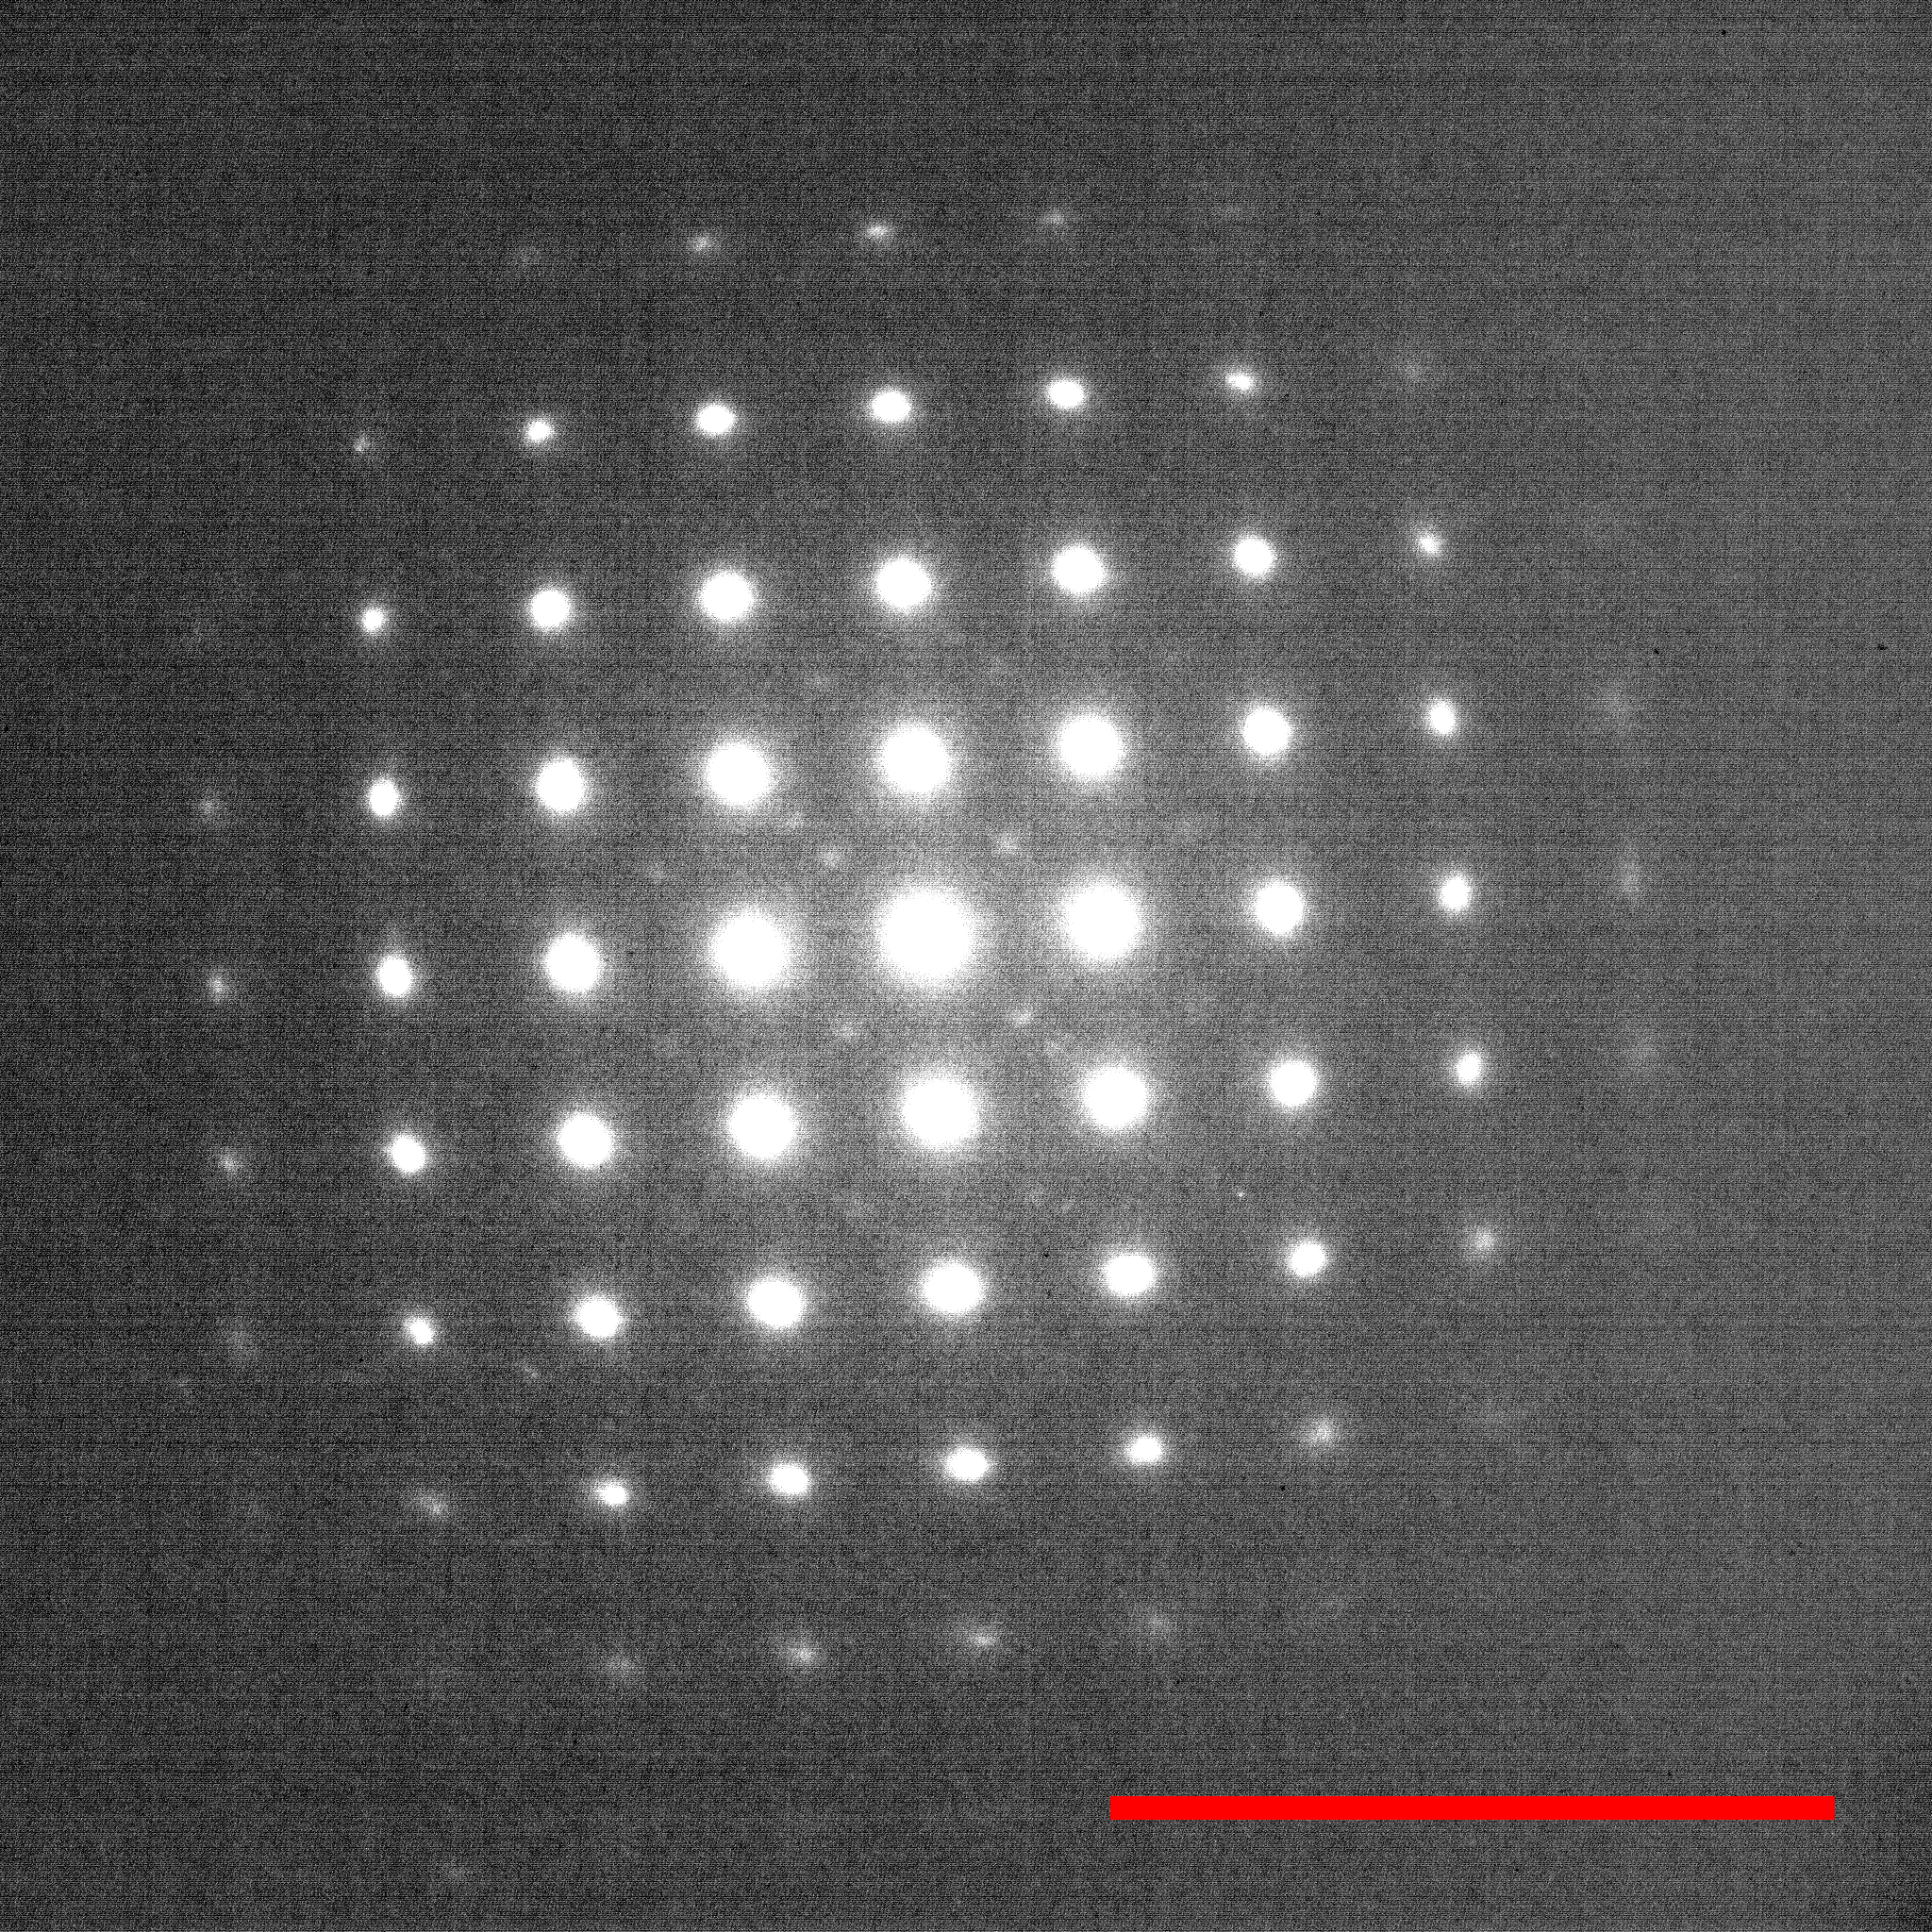
\includegraphics[scale=0.075]{../src/A1/1A-0028.png}}};%
      \begin{scope}[x={(A.south east)},y={(A.north west)}]%
      \filldraw[fill=white,draw=white] (0.572,\barbasel) rectangle node[above] {%
        \footnotesize\color{\col}\SI{20}{\per\nano\metre}} +(0.362,\barthick);%
      \filldraw[fill=white,draw=black]%
        (0.01,0.89) rectangle +(0.1,0.1) node[pos=0.5] {\footnotesize (c)};%
          \node at (0.480,0.515){\tiny{$\cdot$}}; 
          \node at (0.480,0.540){\tiny\color{black}$001$};
          \node at (0.475,0.605){\tiny{$\cdot$}};
           \node at (0.475,0.630){\tiny\color{black}$\bar{1}\bar{1}0_{\alpha}$}; 
          \node at (0.565,0.610){\tiny{$\cdot$}}; 
          \node at (0.600,0.635){\tiny\color{black}$0\bar{2}0_{\alpha}$}; 
          \node at (0.527,0.472){\tiny{$\cdot$}}; 
          \node at (0.562,0.497){\tiny\color{black}$200_{\mathrm{\alpha^{\text{"}}}}$};
      %\subfloat[\label{fig:a1_0028}TEM (DP).]{
      \end{scope}
      \end{tikzpicture}
    };%
    %%%
    \node at (\sqsize,-\sqsize) {%
      \begin{tikzpicture}    
      \node[anchor=south west,inner sep=0] (A) at (0,0) {%
        \fbox{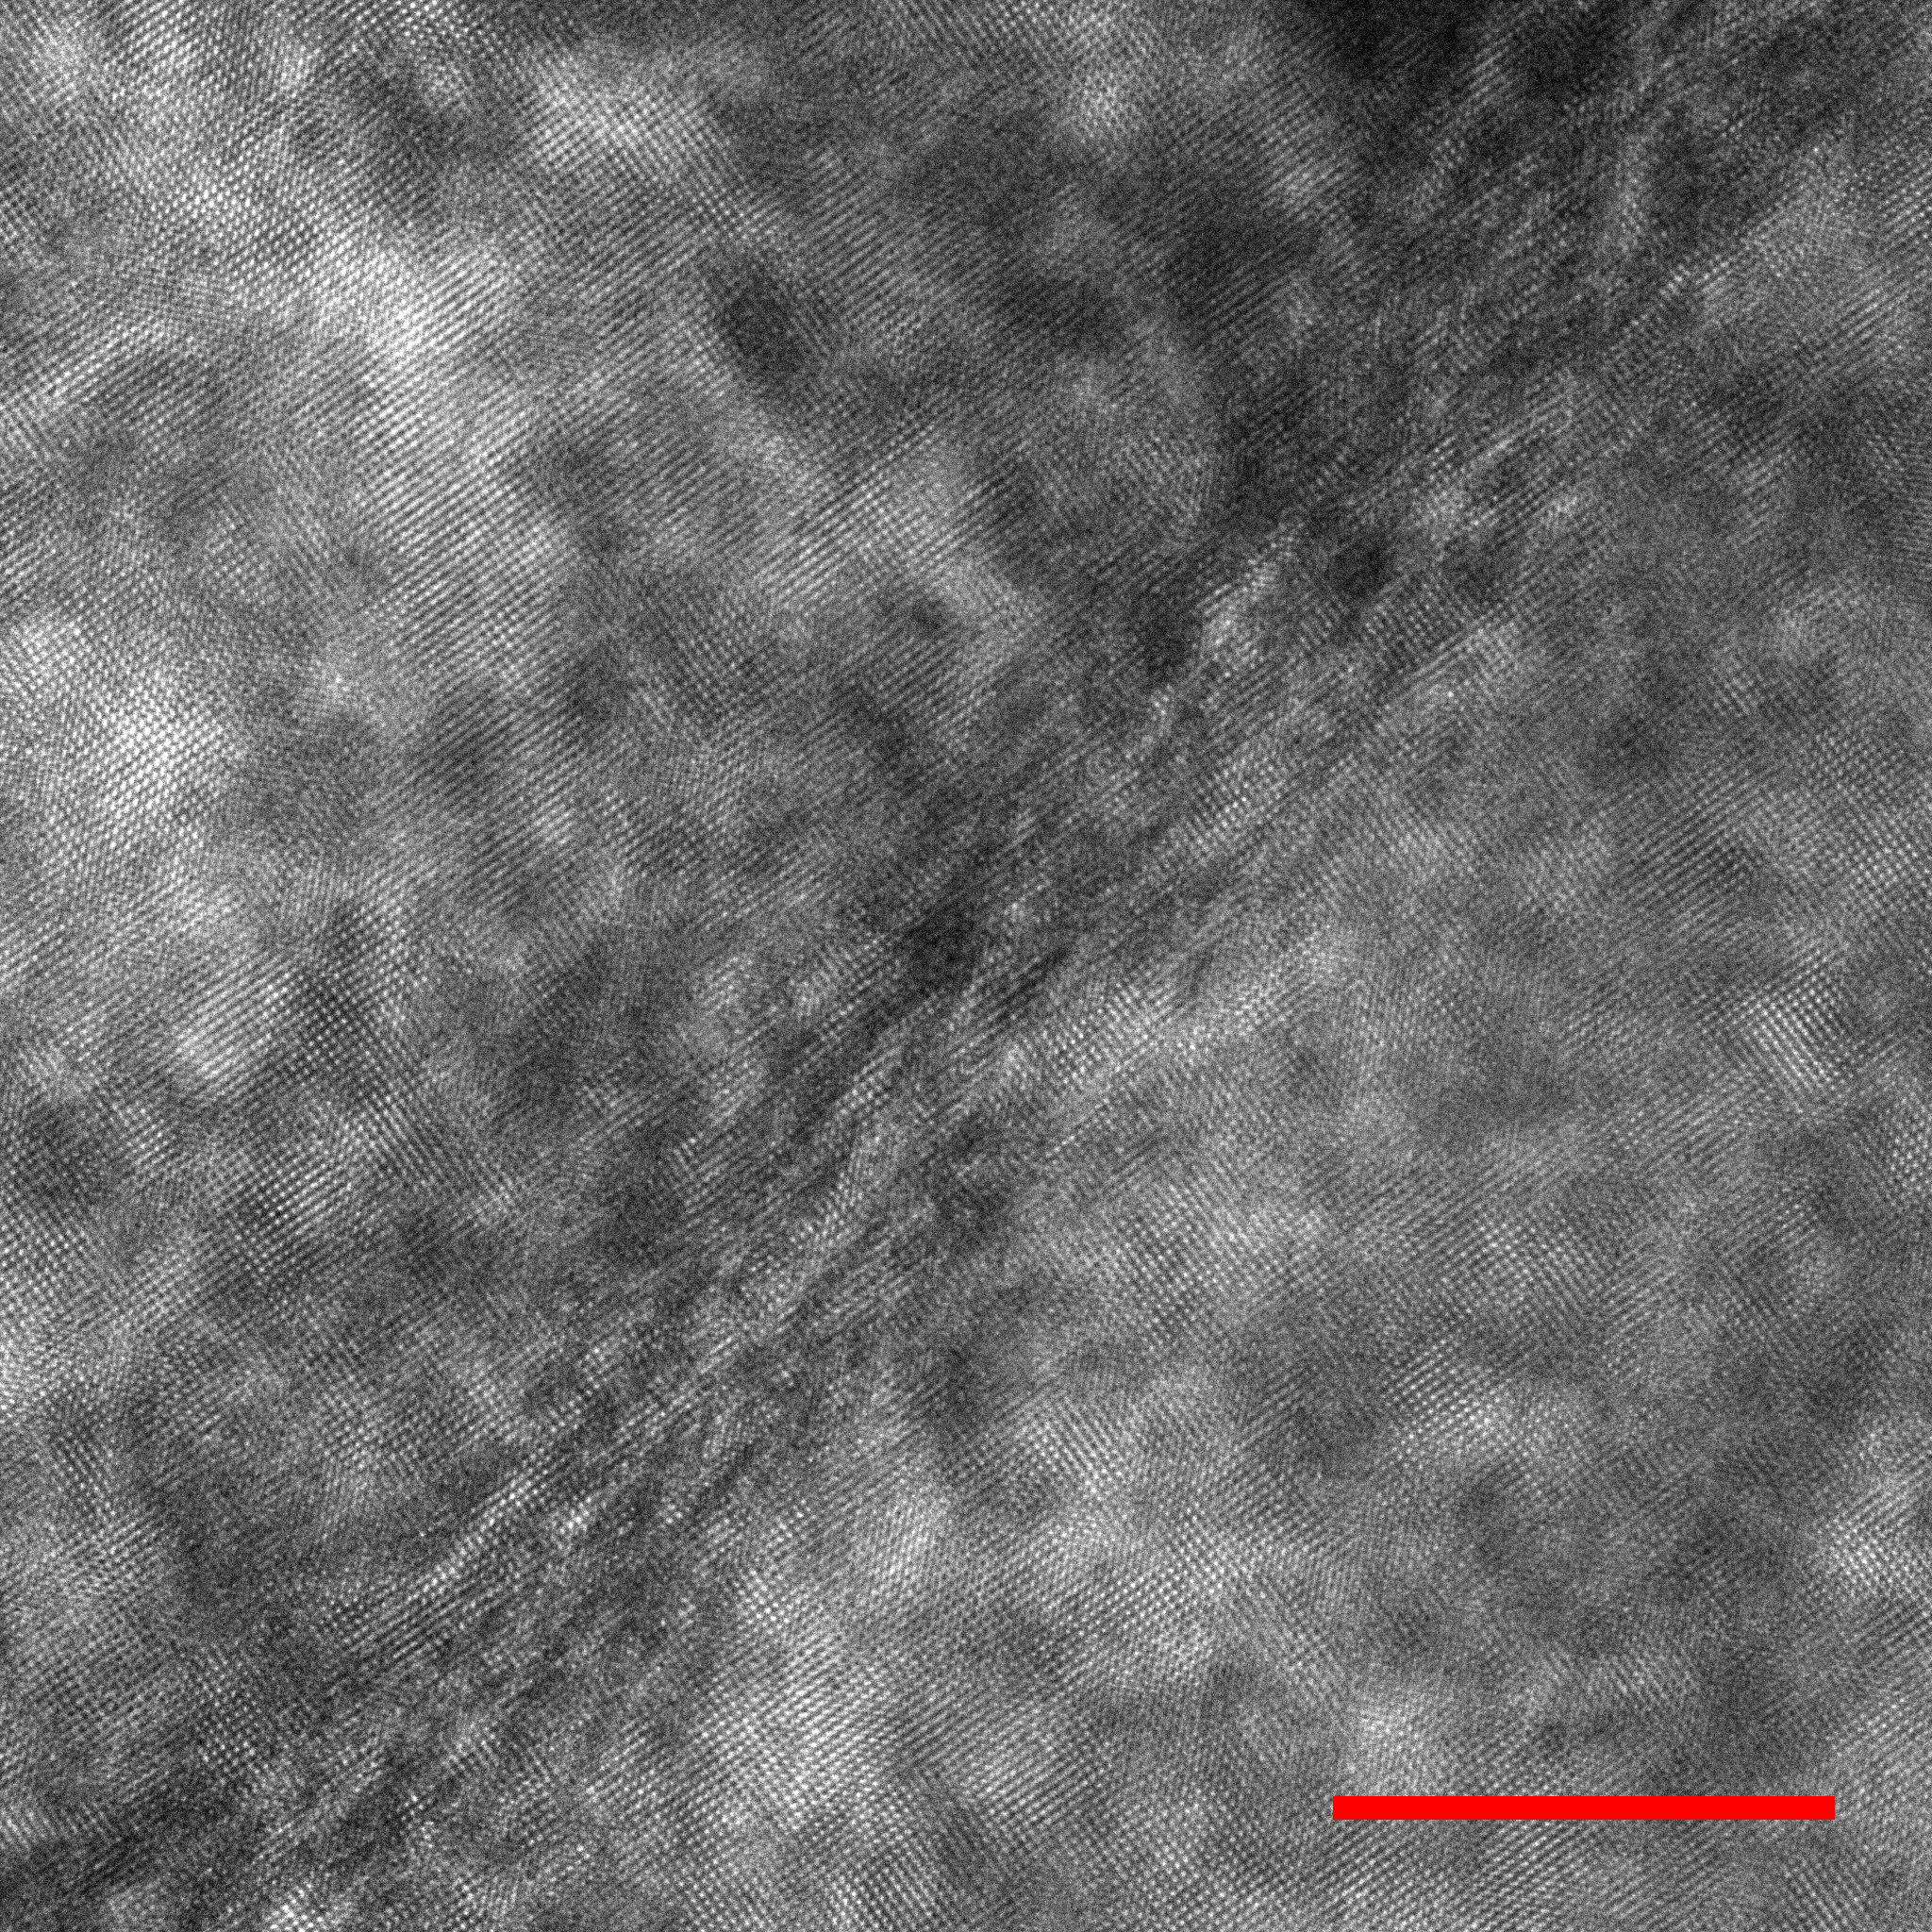
\includegraphics[scale=0.075]{../src/A1/1A-0032.png}}};
      \begin{scope}[x={(A.south east)},y={(A.north west)}]
      \filldraw[fill=white,draw=white] (0.684,\barbasel) rectangle node[above] {
        \footnotesize\color{\col}\SI{10}{\nano\metre}} +(0.25,\barthick);
      \filldraw[fill=white,draw=black] 
      (0.01,0.89) rectangle +(0.1,0.1) node[pos=0.5] {\footnotesize (d)}; 
      %\subfloat[\label{fig:a1_0032}HRTEM $\times$2M.]{
      \end{scope}
      \end{tikzpicture}
    };%
  \end{tikzpicture}
\end{document}